%%%%%%%%%%%%%%%%%%%%%%%%%%%%%%%%%%%%%%%%%%%%%%%%%%%%%%%%%%%%%%%%%%%%%%%%%%%%%
% Баталов Семен, 2021                                                       %
%%%%%%%%%%%%%%%%%%%%%%%%%%%%%%%%%%%%%%%%%%%%%%%%%%%%%%%%%%%%%%%%%%%%%%%%%%%%%

\documentclass[12pt, a4paper]{article}
\usepackage[left=2.5cm, right=2.5cm, top=2.5cm, bottom=2.5cm]{geometry}
\usepackage[utf8]{inputenc}
\usepackage{graphicx}
\graphicspath{{./pictures/}}
\usepackage[english, russian]{babel}
\usepackage{indentfirst}
\usepackage{misccorr}
\usepackage{amsmath}

\title{Задача дискретной классификации для Iris flower data set.}
\author{Баталов Семен}
\date{18.02.2021}

\begin{document}
    
    \sloppy
    
    \maketitle
    
    \section{Iris flower data set}
    
    Это стандартный набор данных, интегрированнный в модуль <<\textbf{sklearn}>> 
    языка <<\textbf{Python}>> (Рис.~\ref{image1}). Набор данных состоит из 150 
    образцов каждого из трех видов ириса (Iris setosa, Iris virginica и Iris 
    versicolor). Для каждого образца были измерены четыре характеристики: длина и 
    ширина чашелистиков и лепестков в сантиметрах. Основываясь на комбинации этих 
    четырех характеристик, можно разработать несложный классификатор, чтобы отличать 
    виды друг от друга.
    
    \begin{figure} [h]
        \center{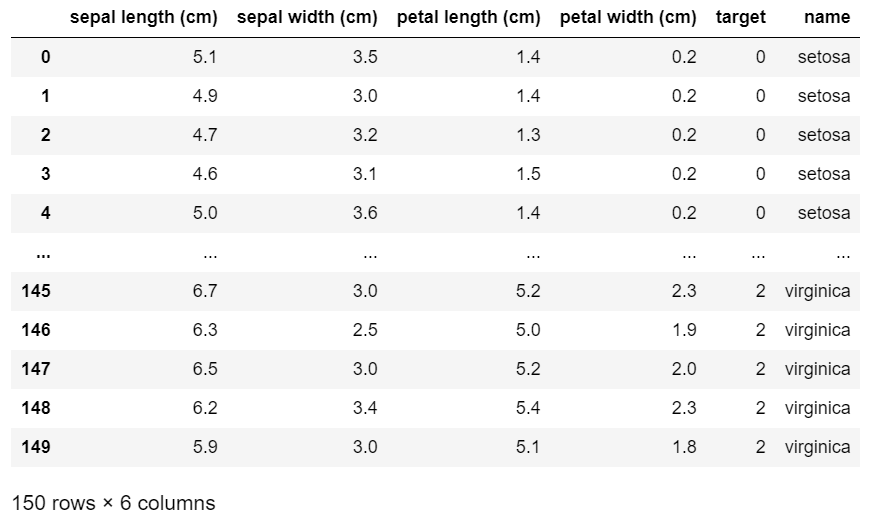
\includegraphics[width = 13cm]{iris_data_set.png}}
        \caption{Набор данных трех видов ириса.}
        \label{image1}
    \end{figure}
    
    \section{Классификатор}
    
    Классификатор был написан на языке <<\textbf{Python}>>. Подробнее о программе можно узнать в папке <<\textbf{source}>> проекта.
    
    При построении дерева (Рис.~\ref{image2}) использовался стандартный 
    классификатор <<\textbf{DecisionTreeClassifier}>> модуля <<\textbf{sklearn}>>. 
    Обучающая выборка составила 50\% от всех полей (переставленных в случайном 
    порядке) в наборе.
    
    \begin{figure} [h]
        \center{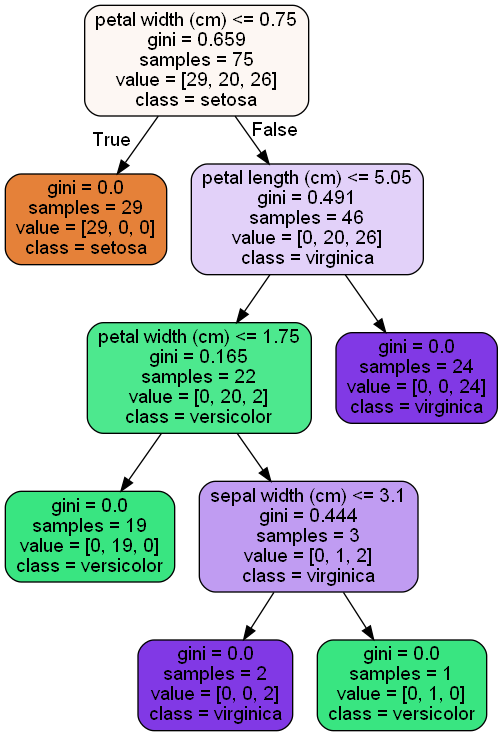
\includegraphics[width = 10cm]{tree.png}}
        \caption{Дерево классификации.}
        \label{image2}
    \end{figure}
    
    После была произведена проверка работоспособности классификатора на оставшихся в датасете примерах. Результат проверки изображен на рисунке (Рис.~\ref{image3}).
    
    \begin{itemize}
        \item \textbf{accuracy}~--~это главная метрика, которая показывает долю 
        правильных ответов модели. Ее значение равно отношению числа правильных 
        ответов, которые дала модель, к числу всех объектов. Но она не полностью 
        отражает качество модели. Поэтому вводятся \textbf{precision} и 
        \textbf{recall}.
        
        \item \textbf{precision}~--~эта метрика показывает, насколько мы можем 
        доверять модели, другими словами, какое у нас количество <<ложных 
        срабатываний>>. Значение метрики равно отношению числа ответов, которые 
        модель считает правильными, и они действительно были правильными (это 
        число обозначается <<true positives>>) к сумме <<true positives>> и числа 
        объектов которые модель посчитала правильными, а на самом деле они были 
        неправильные (это число обозначается <<false positives>>). В виде формулы: 
        precision = <<true positives>> / (<<true positives>> + <<false 
        positives>>).
        
        \item \textbf{recall}~--~эта метрика показывает насколько модель может 
        вообще обнаруживать правильные ответы, другими словами, какое у нас 
        количество <<ложных пропусков>>. Ее численное значение равно отношению 
        ответов, которые модель считает правильными, и они действительно были 
        правильными к числу всех правильных ответов в выборке. В виде формулы: 
        recall = <<true positives>> / <<all positives>>.
        
        \item \textbf{f1-score}~--~это объединение \textbf{precision} и 
        \textbf{recall}.
        
        \item \textbf{support}~--~это просто число найденных объектов в классе.
    \end{itemize}
    
    \begin{figure} [h]
        \center{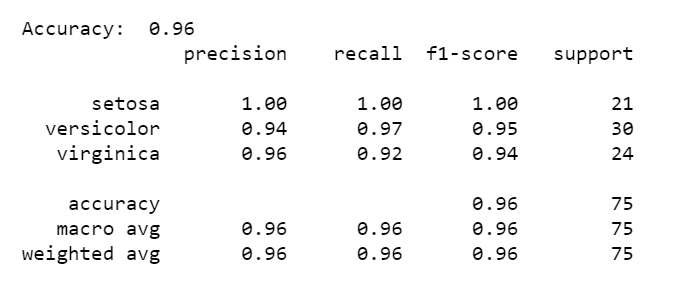
\includegraphics[width = 13cm]{accuracy.png}}
        \caption{Оценка работы классификатора.}
        \label{image3}
    \end{figure}
    
\end{document}